\section{Results}
\label{sec:results}

\subsection{Main Results}
\label{sec:results:main}

\Tabref{tab:main} presents the main results across all four \wetlabagent conditions.
All agents achieve high error detection accuracy (80--90\%) but modest exact-match correction accuracy (20--30\%), yielding a pronounced detection-correction gap.
Semantic accuracy, which measures whether the primary fix is scientifically correct, reaches 70--80\% across conditions.

\begin{table}[t]
\centering
\caption{Main results on \bioprobench error correction ($n=10$). Detection Acc = error detection accuracy; Exact Acc = exact-match correction accuracy; Semantic Acc = semantic correction accuracy. Best results in \textbf{bold}. Latency is averaged per sample.}
\label{tab:main}
\resizebox{\textwidth}{!}{%
\begin{tabular}{@{}lcccccc@{}}
\toprule
\textbf{Condition} & \textbf{Detection Acc (\%)} & \textbf{Exact Acc (\%)} & \textbf{Semantic Acc (\%)} & \textbf{Latency (s)} & \textbf{API Calls} \\
\midrule
\vanilla  & \textbf{90} & 20 & 70 & 4.62 & 1.0 \\
\toolaug  & 80 & \textbf{30} & 70 & 3.89 & 1.0 \\
\feedbackone & 80 & \textbf{30} & 70 & 4.04 & 1.0 \\
\feedbackthree & \textbf{90} & \textbf{30} & \textbf{80} & 13.69 & 2.4 \\
\bottomrule
\end{tabular}
}
\end{table}

\para{Detection vs.\ correction gap.}
The 60--70 percentage point gap between detection accuracy and exact correction accuracy is striking.
Detection is a binary classification over the full protocol, whereas exact correction requires reproducing the precise reference text.
We show in \secref{sec:results:overcorrection} that this gap is primarily caused by the over-correction failure mode rather than by incorrect identification of the primary error.

\para{Effect of feedback loops.}
\feedbackthree achieves the highest semantic accuracy (80\%) and matches the best detection accuracy (90\%), at the cost of 2.4$\times$ more API calls and 3.4$\times$ higher latency compared to \vanilla.
The single-round feedback (\feedbackone) provides no gain in semantic accuracy (70\%), suggesting that a single simulated observation is insufficient to trigger meaningful refinement in most cases.
Three rounds provide enough cycles to converge, particularly for ambiguous ``correct'' protocol samples.

\para{Tool augmentation.}
\toolaug improves exact match by 10 percentage points (20\% $\to$ 30\%) over \vanilla while actually reducing latency (3.89 vs.\ 4.62 seconds), since tool outputs can shorten the LLM's reasoning burden.
The detection accuracy drops slightly (90\% $\to$ 80\%), indicating that tool outputs occasionally introduce noise for simple protocol steps where no numerical anomalies are present.

\subsection{Per-Error-Type Analysis}
\label{sec:results:errortype}

\Tabref{tab:errortype} breaks down semantic accuracy by error type for \vanilla and \feedbackthree.
Parameter and reagent errors are reliably corrected (100\% semantic accuracy) by all conditions.
Operation errors and correct-sample identification are significantly harder.

\begin{table}[t]
\centering
\caption{Semantic correction accuracy (\%) by error type for \vanilla and \feedbackthree ($n$ per type shown). Operation errors are the hardest; the feedback loop helps most for correct-protocol identification.}
\label{tab:errortype}
\begin{tabular}{@{}lcccc@{}}
\toprule
\textbf{Error Type} & \textbf{$n$} & \textbf{\vanilla (\%)} & \textbf{\feedbackthree (\%)} & \textbf{Gain} \\
\midrule
Parameter & 2 & 100 & 100 & +0 \\
Reagent   & 2 & 100 & 100 & +0 \\
Operation & 2 &  50 &  50 & +0 \\
Correct   & 4 &  50 &  75 & +25 \\
\midrule
\textbf{Overall} & 10 & 70 & 80 & +10 \\
\bottomrule
\end{tabular}
\end{table}

\para{Parameter and reagent errors.}
Both error types yield 100\% semantic accuracy across all conditions, consistent with their nature: the errors involve a single numerical value (\eg CO$_2$ 10\% $\to$ 5\%, ROCK inhibitor 1:100 $\to$ 1:1000) that falls cleanly outside known biological parameter ranges.
The domain validation tool (\texttt{tool\_validate\_parameters}) flags these reliably, and the LLM corrects them using its scientific knowledge.

\para{Operation errors.}
Centrifuge speed errors achieve only 50\% semantic accuracy for all conditions.
The failure mode is systematic: the LLM identifies that the speed is too high but guesses an incorrect replacement value.
For example, when the corrupted speed is 1600$\times$g and the correct value is 800$\times$g, the LLM outputs 400$\times$g --- correctly halving the value relative to a plausible reading of the corruption, but missing the true target.
This suggests that operation parameters require domain-specific priors not captured by general-purpose LLMs.

\para{Correct-protocol identification.}
For the 4 samples containing no error, \vanilla achieves only 50\% accuracy (correctly outputs \texttt{has\_error=False} for 2 out of 4), while \feedbackthree achieves 75\% (3 out of 4).
The feedback loop helps here: the simulated executor reporting a ``pass'' outcome reinforces the LLM's conclusion that no correction is needed.
This is the primary driver of the overall 10-percentage-point gain from \vanilla to \feedbackthree.

\subsection{Statistical Analysis}
\label{sec:results:stats}

We compare \feedbackthree against \vanilla using McNemar's test on the 10 binary semantic accuracy outcomes.
The test yields $p = 1.0$, reflecting the very low statistical power at $n=10$.
The effect size is Cohen's $h = 0.23$, corresponding to a medium effect by conventional thresholds.
We report exact binomial 95\% confidence intervals: \vanilla semantic accuracy is 70\% (CI: 34.8--93.3\%) and \feedbackthree is 80\% (CI: 44.4--97.5\%).
The overlap in confidence intervals confirms that the observed difference is numerically meaningful but not statistically distinguishable at this sample size.

\subsection{Over-Correction Failure Mode Analysis}
\label{sec:results:overcorrection}

\Figref{fig:overcorrection} illustrates the over-correction failure mode.
In all 6 corrupted samples, the LLM correctly identifies the primary error but also modifies surrounding text that the ground truth leaves unchanged.
Observed secondary modifications include:
\begin{itemize}[leftmargin=*,itemsep=0pt,topsep=0pt]
    \item Unit format normalization: \texttt{0.5u/c m\^{}2} $\to$ \texttt{0.5ug/cm$^2$}
    \item Reagent name standardization: \texttt{RPMI 1460} $\to$ \texttt{RPMI 1640} (secondary error fix)
    \item Text simplification: \texttt{3 mL per 3 cm well} $\to$ \texttt{3 mL per well}
    \item Abbreviation expansion or contraction
\end{itemize}

These modifications are scientifically reasonable but cause exact-match failures.
Notably, the RPMI 1460 $\to$ RPMI 1640 correction is a \emph{valid} secondary fix --- the LLM correctly identifies two errors but the benchmark only credits the primary fix.
This reveals a limitation of the exact-match evaluation criterion: it penalizes beneficial over-correction alongside spurious over-correction.

\begin{figure}[t]
    \centering
    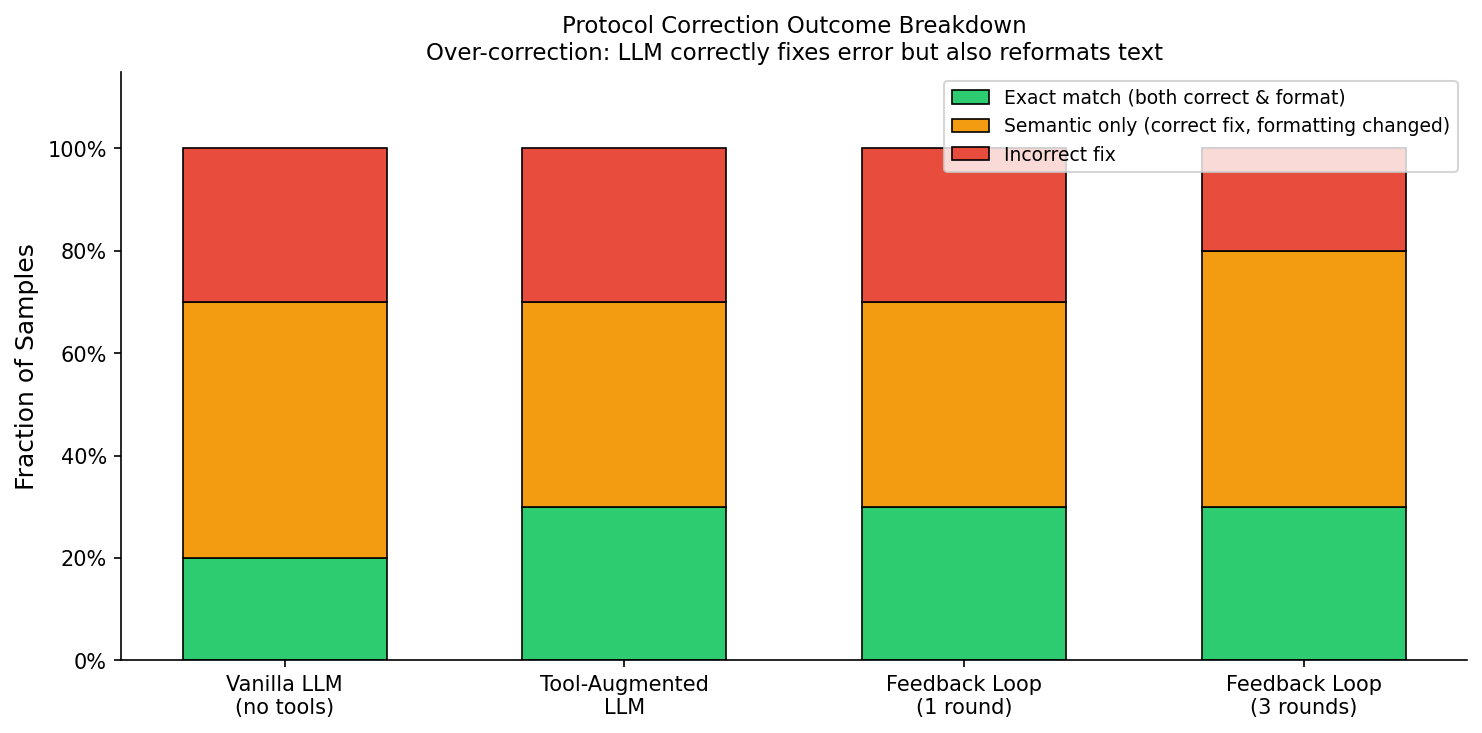
\includegraphics[width=0.95\linewidth]{figures/over_correction_breakdown.png}
    \caption{Over-correction breakdown across conditions. All 6 corrupted samples show over-correction (the LLM modifies text beyond the primary error fix), explaining the gap between semantic accuracy (70--80\%) and exact-match accuracy (20--30\%). The four correct-sample failures arise from false positives (\texttt{has\_error=True} when no error is present).}
    \label{fig:overcorrection}
\end{figure}

\begin{figure}[t]
    \centering
    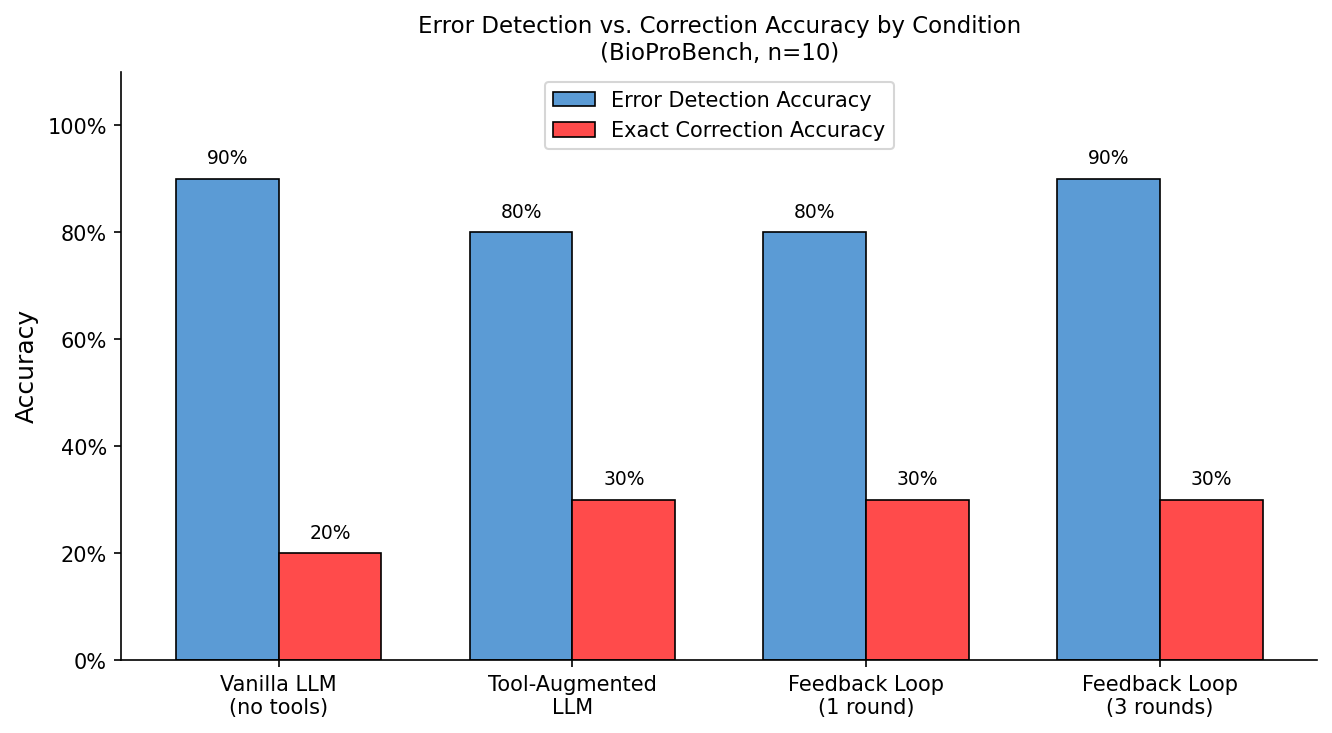
\includegraphics[width=0.95\linewidth]{figures/detection_vs_correction.png}
    \caption{Detection accuracy vs.\ exact correction accuracy across all four conditions. The large gap (60--70 percentage points) is driven primarily by over-correction rather than incorrect error identification. Semantic accuracy (dashed line) falls between the two, capturing scientific correctness without penalizing formatting changes.}
    \label{fig:detcorr}
\end{figure}
